\documentclass[12pt]{article}
\usepackage{graphicx}
\usepackage{amsmath}

\begin{document} 

\title{Summary of Draca et al (2010)}
\author{Thomas Barks}

\maketitle

\section{Introduction}

Draca et al (2011) study the impact of minimum wages on firm profitability, and do so by exploiting the changes induced by the introduction of the National Minimum Wage in 1999 in the United Kingdom. They use pre-policy information on the distribution of wages to conduct a difference-in-differences approach. The main finding of the paper is that higher wages reduce firm profitability, especially in industries with higher market power. They find that this is consistent with the “no behavioural response” model (where increases in wages map directly into a fall in profits). Here I provide a brief summary of how Draca et al (2011) set up their analysis and the main conclusions they found.

\section{Theory}

Minimum wages can come about in three ways: (1) National, government legislated (perhaps after consultations with trade unions and employer associations); (2) National, outcome of collective bargaining agreements and extended to all workers and (3) Industry-level minimum resulting from industry-level collective bargaining and extended to all workers in that industry. The NMW introduced in the UK in 1999 takes the form of (1).

The textbook competitive labour market model is shown in Figure 1. It illustrates that a wage floor reduces employment, as it creates excess supply in the labour market. However, the empirical evidence of this effect is mixed. In light of this, Draca et al (2011) look into a possible reason as to why this is. They put forward that higher wage costs are translated into lower profits (and hence no effect on employment).

\section{Motivation and Modelling Strategy}

The following model is taken from Ashenfelter and Smith (1979). The introduction of the minimum wage (M) above the prevailing wage (W) reduces profits by:

\[\Delta\prod=\prod(W,R,P)-\prod(M,R,P)\]

or
 
\[\Delta\prod=-L\Delta W+\frac{1}{2}\frac{\delta L}{\delta W}(\Delta W)^2\]

This can be rewritten as
 
\[\Delta\prod=-WL(\frac{\Delta W}{W}+\frac{\eta}{2}(\frac{\Delta W}{W})^2\]

where WL is the wage bill, the first term inside the brackets is the proportionate change in the wage, and the second term is the impact on labour demand. In a situation of no behavioural response (no impact on labour demand) the second order effect is zero, so:

\[\Delta\prod=-WL\frac{\Delta W}{W}\]

The previous equations show that the lower the initial wage, the greater the fall in profits. The difference-in-difference model defines treatment groups of more affected firms (lower W) and control groups of less affected firms (higher W). The change in profit margin is:

\[\Delta(\frac{\prod}{S})=-\theta(\frac{\Delta W}{W})\]

In perfect competition, price equals marginal cost, so higher wages translate into higher prices. In oligopoly models higher wages are partly born by firms. The empirical work in the paper distinguishes between industries with different degrees of product market competition (larger effect in less competitive industries).

Now we turn to the modelling the paper used. T=1 for firms whose pre-policy wage was lower than the minimum wage and T=0 for firms whose pre-policy wage was higher than the minimum wage. NMW=1 pre-policy, NMW=0 post-policy and w=ln(W). The wage impact is hence:
 
\[(w_{NMW=1}^{T=1}-\=w_{NMW=0}^{T=1})-(w_{NMW=1}^{T=0}-w_{NMW=0}^{T=0})\]

The regression form is: 

\[w_{it}= \alpha_1+ \beta_1X_{it}+ \delta_1Y_t+ \theta_1I(w_{i,t-1}<mw_t)+ \psi_1[I(w_{i,t-1}<mw_t)NMW_t]+ \varepsilon_{1it}\]

$\psi_1$ shows the estimated impact of the NMW on wages. The profit margin impact is:

\[[(\frac{\prod}{S})_{NMW=1}^{T=1}-(\frac{\prod}{S})_{NMW=0}^{T=1}]-[(\frac{\prod}{S})_{NMW=1}^{T=0}-(\frac{\prod}{S})_{NMW=0}^{T=0}]\]

The regression form is:

\[(\frac{\prod}{S})_{it}= \alpha_2+ \beta_2Z_{it}+ \delta_2Y_t+ \theta_2I(w_{i,t-1}<mw_t)+ \psi_2[I(w_{i,t-1}<mw_t)NMW_t]+ \varepsilon_{2it}\]

$\psi_2$ shows the estimated impact of the NMW on profit margins.

\section{Data}

The paper uses the FAME (Financial Accounting Made Easy) database. This was used as it covers a wider range of companies than standard. This is of particular importance, as smaller firms and non-manufacturing firms are more likely to employ workers whose wages were at or below the minimum wage level. The paper also used the LFS (Labour Force Survey) for control variables and the WERS (Workplace Employment Relations Survey) to construct and validate treatment group indicators. To summarise, FAME was used for the main results and average firm wages, LFS was used for industry-level analysis of entry and exit and WERS was used to see the association between low pay incidence and average wages. T=1: average remuneration <£12,000. The key issue is that wages of firms beneath the threshold have a significant wage boost relative to higher wage firms. This threshold based definition is more effective if sub MW employers are concentrated at the lower end of the wage distribution. Using WERS, the paper found a strong negative relationship between the proportion of workers paid below £3.60 per hour and the establishment average wage per hour. Workplaces with average annual wages less than or equal to £12,000 contain 87 percent of all minimum wage workers, as Figure 2 illustrates. 

\section{Conclusion}

The main finding of the paper is that wages were significantly raised and firm profitability was significantly reduced due to the NMW. There was also some evidence of bigger falls in profit margins for industries with higher market power, but no effects on employment or productivity. These findings were found to be consistent with a simple no behavioural response model. In addition, long run adjustment may be through lower rates of entry. A positive of the paper is that it covered an under-studied research question. Furthermore, the models used were relatively straightforward. Also, robustness checks found significant results. However, the authors could not find any data on prices and quality, variables which could also change due to the NMW. In addition, there was limited information on the within-firm distribution of workers in sectors besides care homes. Lastly, the paper could have perhaps explained how the government decided on the value of the NMW. 

\begin{figure}
	\centering 
	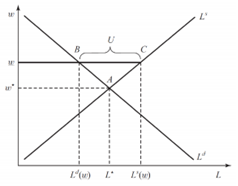
\includegraphics{NC}
	\caption{Competitive Labour Market}
\end{figure} 

\begin{figure}
	\centering
	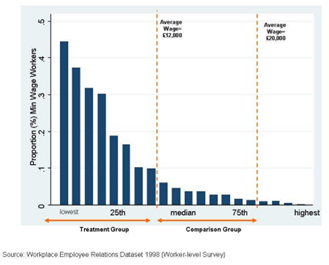
\includegraphics{NC1}
	\caption{Wage Distribution}
\end{figure} 

\end{document} 